\documentclass[12pt,a4paper]{article}
\usepackage[brazilian]{babel}
\usepackage[utf8]{inputenc}
\usepackage[T1]{fontenc}
\usepackage{amsmath,amssymb}
\usepackage{graphicx}
\usepackage{geometry}
\usepackage{hyperref}
\geometry{margin=2.5cm}

\title{Aula 05 - Expansao de Taylor\\Resumo, Exemplo e Exercicios Resolvidos}
\author{Baseado apenas nos arquivos da pasta 4}
\date{14/04/2026}

\begin{document}
\maketitle

\section{Resumo rapido}
O PDF da pasta 4 traz o tema de metodos de modelagem e solucao numerica. No contexto da aula de expansao de Taylor, os pontos fundamentais sao:
\begin{itemize}
  \item aproximar funcoes por polinomios locais;
  \item controlar erro de truncamento;
  \item usar aproximacoes para construir metodos numericos.
\end{itemize}

\section{Explicacao simples}
A expansao de Taylor troca uma funcao complicada por um polinomio perto de um ponto.
Quanto mais termos usamos, melhor a aproximacao (em geral, perto do ponto de expansao).
Isso e muito util para calcular rapidamente e para montar metodos numericos.

\section{Exemplo guiado}
Maclaurin de $e^x$ ate ordem 3:
\begin{equation}
e^x\approx 1+x+\frac{x^2}{2}+\frac{x^3}{6}.
\end{equation}
Para $x=0.2$:
\begin{equation}
e^{0.2}\approx 1.221333,
\end{equation}
valor muito proximo do real.

\section{Exercicios dos slides resolvidos passo a passo}
\subsection*{Exercicio 1: Maclaurin de $e^x$ ate ordem 3}
\begin{equation}
e^x \approx 1 + x + \frac{x^2}{2} + \frac{x^3}{6}.
\end{equation}
Para $x=0.2$:
\begin{equation}
e^{0.2} \approx 1 + 0.2 + 0.02 + 0.001333 = 1.221333.
\end{equation}
Valor real: $1.22140\ldots$ (erro pequeno).

\subsection*{Exercicio 2: aproximacao de $\sin x$ para angulos pequenos}
\begin{equation}
\sin x = x - \frac{x^3}{6} + \mathcal{O}(x^5).
\end{equation}
Logo, para $|x|\ll 1$:
\begin{equation}
\sin x \approx x.
\end{equation}

\begin{figure}[htbp]
\centering
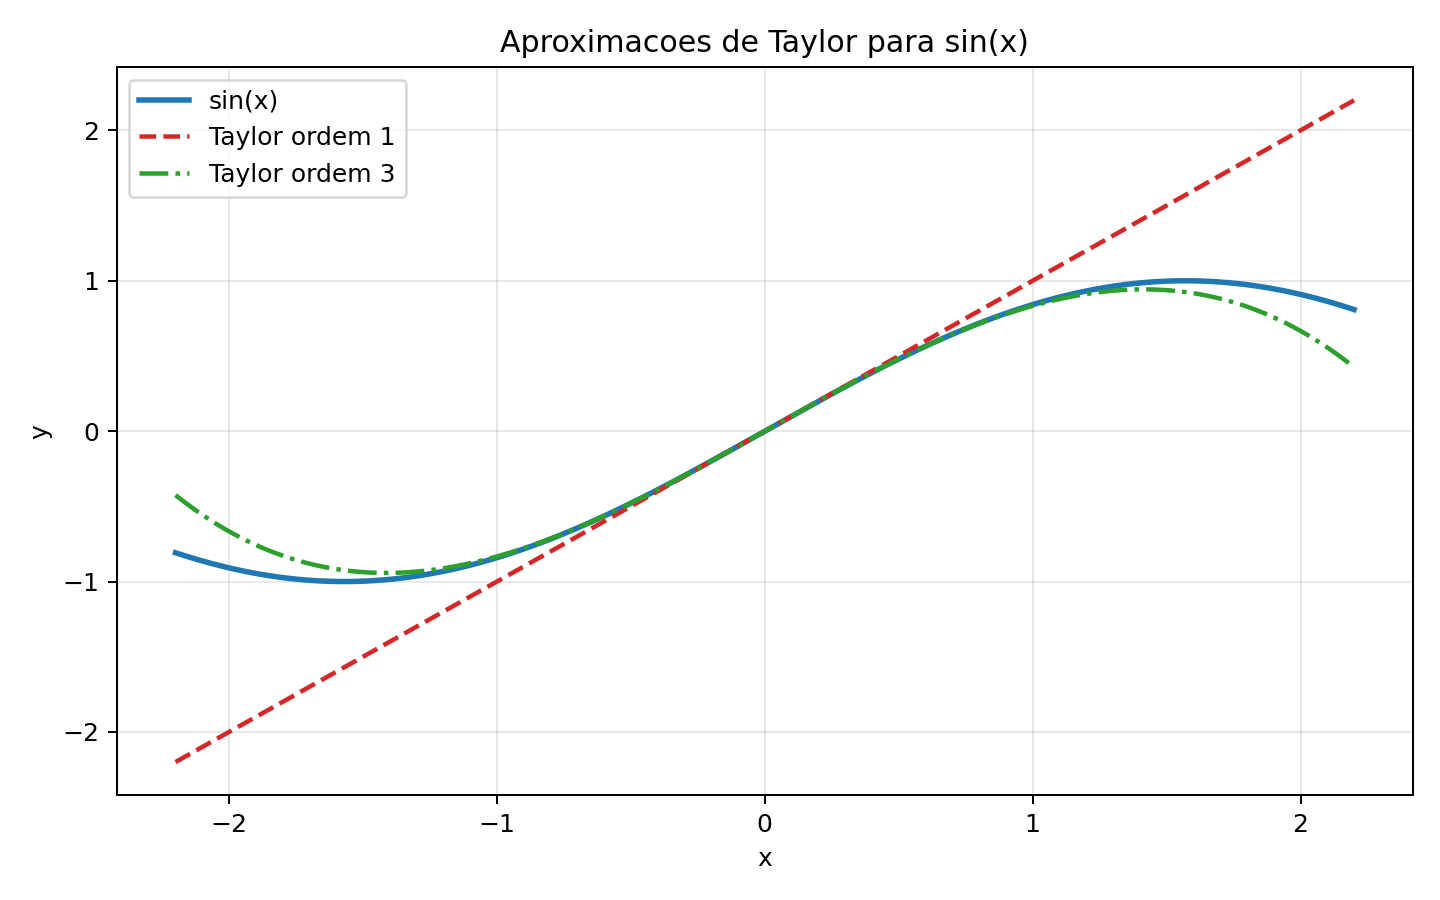
\includegraphics[width=0.8\textwidth]{figuras/taylor_seno.png}
\caption{Comparacao entre $\sin(x)$ e aproximacoes de Taylor (ordens 1 e 3).}
\end{figure}

\subsection*{Exercicio 3: Taylor de $\ln(1+x)$ ate ordem 2}
\begin{equation}
\ln(1+x) \approx x - \frac{x^2}{2}.
\end{equation}
Para $x=0.1$:
\begin{equation}
\ln(1.1) \approx 0.1 - 0.005 = 0.095.
\end{equation}
Valor real: $0.09531\ldots$.

\section{Conexao com metodos numericos}
A expansao de Taylor justifica o metodo de Euler:
\begin{equation}
y(t+\Delta t)=y(t)+y'(t)\Delta t + \mathcal{O}(\Delta t^2).
\end{equation}
Ao truncar termos de ordem superior:
\begin{equation}
y_{n+1}=y_n+f(t_n,y_n)\Delta t.
\end{equation}

\section{Fontes web para revisar}
\begin{itemize}
  \item Serie de Taylor (definicao e series classicas): \url{https://pt.wikipedia.org/wiki/S%C3%A9rie_de_Taylor}
\end{itemize}

\end{document}
